\section{Software}

\subsection{Regelung}
Die Software zur Regelung beinhaltet zwei Integer-Arrays, $sauber[]$ und $verschmutzt[]$, welche mittels der Headerdatei $LookUpTable.h$ geladen werden. In diesen beiden Arrays sind die Spannungswerte in Millivolt für die saubere und die schmutzige Solarzelle hinterlegt, jeweils ein Wert alle 10 Milliampere. Der Index entspricht dabei dem jeweiligen Stromwert geteilt durch 10. \newline
Die Werte dazu wurden mittels eines Matlab-Files erstellt, das im Anhang angehängt ist. Die Werte entsprechen dabei der in Formel (\ref{eq:kennlinie}) berechneten Kennlinie.

Im Programm selbst gibt es die Integer $prozent$, welche die aktuelle Bestrahlungsstärke darstellt, und $regelwert$, welcher angibt, wie stark der Regler korrigieren soll. \newline
In der Funktion $main$ existieren ausserdem die Integer $messU$ für die gemessene Spannung am Spannungsteiler, $istU$ für die berechnete Ausgangsspannung, $sollU$ für den zum Stromwert passenden Spannungswert, $messI$ für die gemessene Spannung am Eingang des Controllers für die Strommessung und $istI$, worin der berechnete Ausgangsstrom gespeichert ist. Sämtliche Variabeln repräsentieren dabei die Werte in Millivolt bzw. Milliampere. \newline
Zur Realisierung der Umschaltung zwischen sauber und verschmutzt ist ausserdem noch der Integer $modus$ vorhanden. Dieser kann die beiden Zustände $MODUSSAUBER$ (entsprechend einer 1) und $MODUSVERSCHMUTZT$ (entsprechend einer 0) annehmen.

\begin{figure}[h]
	\centering
		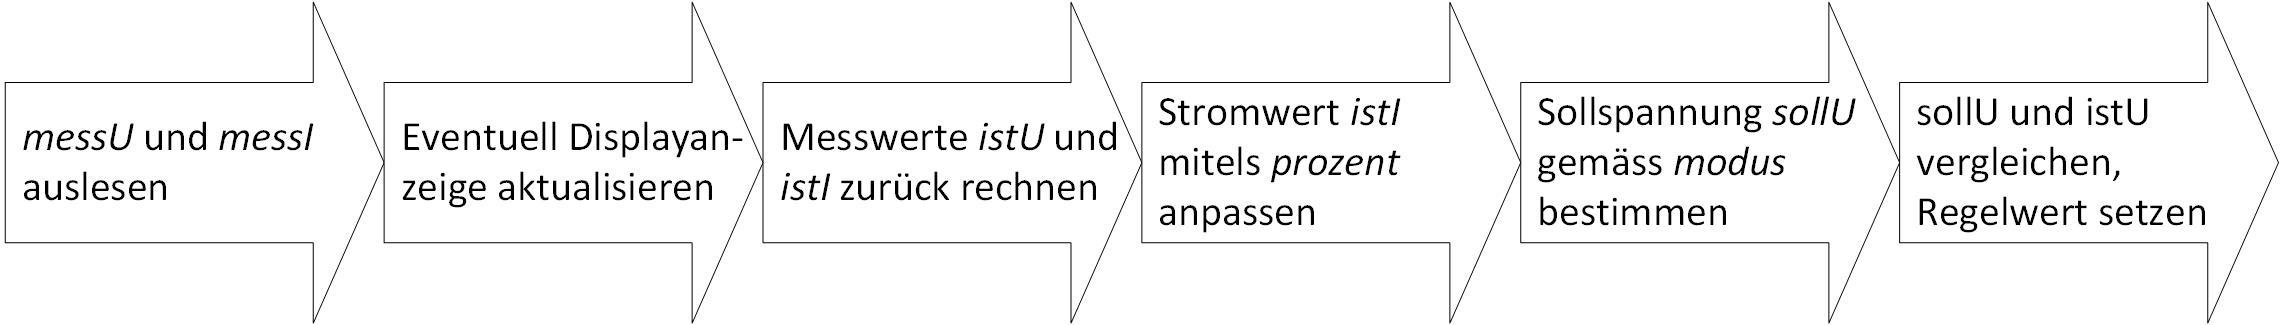
\includegraphics[width=1.00\textwidth]{Pfeildiagramm_Software.jpg}
	\caption{Flussdiagramm der Regelungsroutine.}
	\label{fig:Pfeildiagramm_Software}
\end{figure}

Abbildung \ref{fig:Pfeildiagramm_Software} zeigt als Flussdiagramm den Ablauf der Regelungssoftware, welche nachfolgend erläutert wird. Die Routine zur Regelung wird mittels einem Vergleich ausgeführt, welcher sich alle \colorbox{red}{1ms (eventuell nachträglich anpassen} wiederholt. Dabei werden zuerst die beiden analogen Eingänge für $messU$ und $messI$ ausgemessen und aus den gemessenen Werten $messU$ und $messI$ die aktuellen Werte am Ausgang des Gerätes $istU$ und $istI$ berechnet. \newline
Anschliessend wird der Wert $istI$ mit der Beleuchtungsstärke $prozent$ verrechnet, um die Kennlinie entsprechend zu verschieben. Wie das genau funktioniert ist im Kapitel \ref{subsec_mathe} ausführlich beschrieben. \newline
Der so erhaltene Wert muss nun auf dem Wertebereich der $LookUpTable.h$ abgeglichen werden. Dazu werden zu grosse oder zu kleine Werte auf den Maximal- beziehungsweise Minimalwert korrigiert und anschliessend die Genauigkeit auf 10 Milliampere angepasst.

Das Programm prüft nun, ob in der Variabel $modus$ der Wert $SAUBER$ oder $VERSCHMUTZT$ hinterlegt ist. Je nachdem welcher Modus gewählt ist wird der Referenzwert für $sollU$ aus dem Array $sauber[]$ oder $verschmutzt[]$ geladen. Die Indexposition entspricht dabei dem oben angepassten Wert des Stromes $istI$. Der Spannungswert von $sollU$ entspricht nun der Spannung, welche bei diesem Strom gemäss der Formel (\ref{eq:kennlinie}) auftreten sollte.

Der aktuelle Spannungswert am Ausgang $istU$ wird nun mit dem Referenzwert $sollU$ verglichen. Falls $istU$ grösser als $sollU$ ist, wird $regelwert$ negativ. Um die Regelung genauer zu gestalten, sind für $regelwert$ zwei mögliche negative Werte möglich: -1 für ein langsames verringern der Spannung und -2 für ein schnelles verringern der Spannung. Zu diesem Zweck wird ein neuer Integer $differenz$ erstellt, welcher die Differenz zwischen $istU$ und $sollU$ beinhaltet. Falls diese Differenz grösser als 200 Millivolt ist, wird die Spannung schnell verringert, also wird für $regelwert$ der Wert -2 gesetzt. Falls dies nicht der Fall ist, wird für $regelwert$ der Wert -1 gesetzt. \newline
Falls $sollU$ grösser als $istU$ ist, wird für $regelwert$ ein positiver Wert gesetzt, der ebenfalls zwei Abstufungen kennt. Dies funktioniert jedoch gleich wie bei negativen Werten von $regelwert$. \newline
Falls $sollU$ und $istU$ den selben Wert haben wird für $regelwert$ eine 0 gesetzt. Das bedeutet, dass der Regler selbst nicht verändert werden soll.

\colorbox{red}{Ergänzen um Teil zur Ansteuerung des Reglers (Sturm)}




%Die Software zur Regelung funktioniert nach dem Vergleichsprinzip. Dabei werden zuerst die beiden Messwerte $istI$ und $istU$ auf die Werte in Milliampere bzw. Millivolt genormt. Anschliessend wird der gemessene Strom, welcher im Integer $istI$ gespeichert ist, mittels der Variable $prozent$ auf der Kennlinie verschoben. Das mathematische Vorgehen dazu ist im Kapitel \colorbox{red}{Referenz auf Matheteil}beschrieben.
%
%Der so erhaltene Wert von $istI$ wird mit der Lookup-Table $sauber$ bzw. $verschmutzt$, welche mittels Int-Array realisiert wurde, verglichen. In diesen beiden Arrays ist dabei für alle 10 Milliampere Strom der dazugehörige Spannungswert notiert. Mittels der Zeile $istI=istI/10;$ wird der Wertebereich von $istI$ an die Wertebereiche der Arrays angepasst. Die Entscheidung darüber, mit welchem Array verglichen wird, hängt vom Integer $modus$ ab. Dieser kann die beiden Werte $VERSCHMUTZT$ und $SAUBER$ annehmen.
%
%Die Arrays wurden mittels Matlab erstellt und exportiert. Die so erhaltenen Werte sind in der Headerdatei $LookUpTable.h$ hinterlegt, wobei die Werte jeweils den Kennlinien für 100\% Bestrahlungsstärke entsprechen. Die beiden Arrays entsprechen dabei den beiden Betriebsarten $SAUBER$ ($sauber[])$ und $VERSCHMUTZT$ ($verschmutzt[]$).